\question{Erzwungene, ungedämpfte Schwingung}
\vspace{1em}

     \begin{tikzpicture}[scale=0.6]
 \fill[black!5!white] (-1,-2) rectangle (7, 3); 
\draw[->] (2.5, 2) --(4, 2);
\draw (2.5,1.8) -- (2.5, 2.2);
\draw[thin] (4,1.5)--(4,2.2);
\draw (0, 0) pic [scale=0.6] {DKbase};
\draw (0, 0) pic [scale=0.6, thick] {DKspring=4};  
\draw[thick] (4,-1.5) rectangle +(1.5, 3); 
\draw (2, -0.9) node {$k$};
\draw (4.7, 0) node {$m$};
\draw (3.25, 2.3) node {$u$};
\draw[->, very thick] (5.7, 0) -- (6.9, 0);
\draw (6.25, 0.55) node {$F(t)$};
\end{tikzpicture}


    \begin{minipage}[t]{.49\linewidth}
    geg.:
    \begin{tasks}(2)
        \task[] $m = \SI{3}{\kilo\gram}$
        \task[] $k = \SI{10}{\newton\per\meter}$
        \task[] $F(t) = \hat{F} \sin{\omega t}$
        \task[] $\hat{F} = \SI{5}{\newton}$
        \task[] $\omega = \SI{10}{\radian\per\second}$
        \task[] $t=\SI{0}{\second}$
        \task[] $u_0 = \SI{0.1}{m}$
        \task[] $\dot{u}_0 = \SI{0}{\meter\per\second}$
    \end{tasks}
    \end{minipage}
    \begin{minipage}[t]{.49\linewidth}
    ges.:
    \begin{tasks}
        \task $u(t)$
    \end{tasks}
    \end{minipage}

    \begin{solution}
        \begin{alignat*}{2}
            &(c = \SI{0}{\newton\second\per\meter}, F_C = \SI{0}{\newton}, F_S = \hat{F} = \SI{5}{\newton})\\
            &\omega_0 = \sqrt{k/m} &&= \SI{1.826}{\radian\per\second} \\
            &\zeta = \frac{c}{2\sqrt{mk}} &&= 0 \\
            &\eta = \omega/\omega_0 &&= 5.477\\
            &V = (1-\eta^2)^{-1} &&=  0.0345 \\
            &u_C = -2V^2\zeta\eta\hat{F}/k &&= \SI{0}{\meter} \\
            &u_S = V^2(1-\eta^2)\hat{F}/k &&= \SI{-0.0172}{\meter}
        \end{alignat*}

        \begin{align*}
            u_0 &= C_1 + u_C \\
            \dot{u}_0 &= \omega_0 C_2+\omega u_S\\
            &\rightsquigarrow \\
            C_1 &=  u_0 - U_C = \SI{0.1}{\meter}\\
            C_2 &= \frac{\dot{u}_0 - \omega u_S}{\omega_0} = \SI{0.0944}{\meter} \\
            \vspace{1cm}
        \end{align*}

        \begin{equation*}
            \begin{split}
                u(t) = \SI{0.1}{\meter} \cos{(\SI{1.826}{\radian\per\second} t)} +\SI{0.0944}{\meter} \sin{((\SI{1.826}{\radian\per\second} t))} \\ - \SI{0.0172}{\meter}\sin{(\SI{10}{\radian\per\second} t)}
            \end{split}
        \end{equation*}
            \fbox{\textbf{Anmerkung:} Das Einschwingen dauert im  ungedämpften Fall unendlich lang.}
    \end{solution}
    
%%%%%%%%% Übungsaufgabe 2 %%%%%%%%%

\question{Erzwungene, gedämpfte Schwingung}

    \begin{tikzpicture}[scale=0.6]
\fill[black!5!white] (-1,-3) rectangle (7, 3); 
\draw (0, 0) pic [scale=0.6] {DKbase};
\draw (0, 1) pic [scale=0.6, thick] {DKspring=4};
\draw (0,-1) pic [scale=0.6, thick] {DKdashpot=4};  
\draw[->] (2.5, 2) --(4, 2);
\draw (2.5,1.8) -- (2.5, 2.2);
\draw[thin] (4,1.5)--(4,2.2);
\draw[thick] (4,-1.5) rectangle +(1.5, 3); 
\draw (2.0, 0.1) node {$k$};
\draw (2.0,-1.9) node {$c$};
\draw (4.7, 0) node {$m$};
\draw (3.25, 2.3) node {$u$};
\draw[->, very thick] (5.7, 0) -- (6.9, 0);
\draw (6.25, 0.55) node {$F(t)$};
\end{tikzpicture}


    \begin{minipage}[t]{.49\linewidth}
        geg.:
        \begin{tasks} (2)
           \task[] $m = \SI{3}{\kilo\gram}$
           \task[] $c = \SI{1}{\newton\second\per\meter}$
           \task[] $k = \SI{10}{\newton\per\meter}$
            \task[] $F(t) = \hat{F} \sin{\omega t}$
           \task[] $\hat{F} = \SI{5}{\newton}$
           \task[] $\omega = \SI{10}{\radian\per\second}$
           \task[] $t=\SI{0}{\second}$
           \task[] $u_0 = \SI{0.1}{m}$
           \task[] $\dot{u}_0 = \SI{0}{\meter\per\second}$
           \task[] $t_0 = \SI{0}{\second}$
        \end{tasks}
        \end{minipage}
        \begin{minipage}[t]{.49\linewidth}
        ges.:
        \begin{tasks}
            \task[] $u(t)$
        \end{tasks}
    \end{minipage}\\
    \vspace{1cm}

    \underline{Zusatzfrage:} Wie ändert sich die Lösung, wenn die Anregung zusätzlich einen Konstantanteil enthält $F(t) = F_{DC} +\hat{F} \sin{(\omega t)}$ (Stichwort \textit{statische Ruhelage})?

    \begin{solution}
        \begin{alignat*}{2}
            &\omega_0 = \sqrt{k/m} &&= \SI{1.826}{\radian\per\second} \\
            &\zeta = \frac{c}{2\sqrt{mk}} &&= 0.091 \\
            &\eta = \omega/\omega_0 &&= 5.477\\
            &V = \frac{1}{\sqrt{(1 - \eta^2)^2 + (2\zeta\eta)^2}} &&= 0.034\\
            &\text{da: } a(t) = \frac{F(t)}{k} \sin(\omega t) = \hat{a} \cos(\psi_a) \cos(\omega t) + \hat{a} \sin{\psi_a} \sin{\omega t} \\
            &F_c = 0 && F_s = \SI{5}{\newton} \\
            &a_c = \frac{F_c}{k} &&= \SI{0}{\newton}\\ 
            &a_s = \frac{F_s}{k} &&= 0.2 m^{-1} \\
            &a= a_c \sin(\omega t) + a_s \sin(\omega t) &&= 0 \\
            &\psi = \arctan(\frac{2\zeta \eta}{1-\eta^2}) &&= \SI{3.107}{\radian}\\
            &u_c = V^2((1-\eta^2)a_c - 2 \zeta \eta a_s) &&= \SI{-0.0006}{\meter}\\
            &u_s = V^2((1 - \eta^2)a_s + 2 \zeta \eta a_c) &&= \SI{-0.0172}{\meter}\\
            &u_p(t)= u_c \cos(\omega t) + u_s \sin(\omega t) &&= -0.0006 \cdot \cos{10t} - 0.0172 \cdot \sin{10t}\\
        \end{alignat*}
    \end{solution}
        
%\begin{figure}[h]
    \centering
    \begin{gnuplot}[terminal=epslatex, terminaloptions={size 15cm,5cm}]
       set zeroaxis
       unset border
       set xtics axis
       unset ytics
       unset key

       set xr [0:3*pi]
       set yr [-1:1]
       set xl "t" offset 27,7,0
       set yl "u" offset 2,6,0 rotate by 0

       set xtics ("$t_{max1}$" pi/4, "$t_{max2}$" pi/4+2*pi)

       set label 1 "" at pi/4,1 point pointtype 7 pointsize 2 lc 0
       set label 2 "" at pi/4+2*pi,1 point pointtype 7 pointsize 2 lc 0

       set arrow 1 from 0,0 to graph 0, first 1 filled head
       set arrow 2 from 0,0 to first 0, graph 0 filled head
       set arrow 3 from 0,0 to graph 1,.5 filled head

       plot cos(x-pi/4) w l lc 0
    \end{gnuplot}
\end{figure}


\question{Ausschwingversuch}

    \begin{tikzpicture}
\begin{axis}[
    width=10cm, 
    height=5cm,
    axis x line=center, 
    axis y line=middle, 
    xlabel={$t$},
    x label style={at={(current axis.right of origin)}, right},
    ylabel={$u$},
    y label style={at={(current axis.above origin)}, left},
    samples=100,
    ymin=-1.1, ymax=1.2,
    xmin=0, xmax=11,
    domain=0.2:3.2*pi,
    xtick={ 1.0472, 7.3304 },
    xticklabels={ 
    $t_\mathrm{max1}$, $t_\mathrm{max2}$
    },
    ytick={0},
    yticklabels={}
]
\addplot [mark=none, semithick] {exp(-0.03*x)*cos(deg(x)-60)};
\fill (axis cs: 1.0472, 0.975) circle [radius=1mm];
\fill (axis cs: 7.3304, 0.81) circle [radius=1mm];
\end{axis}
\end{tikzpicture}


    \begin{minipage}[t]{.49\linewidth}
        geg.:
        \begin{tasks} (1)
           \task[] $m = \SI{3}{\kilo\gram}$
           \task[] $u(t_{max1}) = \SI{0.10}{\meter}$
           \task[] $u(t_{max2}) = \SI{0.08}{\meter}$
           \task[] $T_{id} = t_{max2}-t_{max1} = 1$
           \task[] $N = 1$
        \end{tasks}
        \end{minipage}
        \begin{minipage}[t]{.49\linewidth}
        ges.:
        \begin{tasks}
            \task$c ~,~ k$
        \end{tasks}
    \end{minipage}\\
    \vspace{1cm}

    \fbox{\underline{Hinweis:} Nutzen Sie das logarithmische Dekrement $\Lambda = \log \frac{u(t_{max1})}{u(t_{max2})}$ als Zwischenergebnis.}

    \begin{solution}
        \begin{alignat*}{2}
            &\omega_{1_{id}} = \frac{2 \pi}{T_{id}} &&= 2 \pi\\
            &\Delta_{id} = \frac{1}{N \cdot T_{id} } \cdot \ln{\frac{u_1}{u_2}} &&= 0.223\\
            &c_{id} = 2 \cdot \Delta_{id} \cdot m &&= \SI{1.339}{\newton \second \per \meter}\\
            &\omega_{0_{id^2}} = \omega_{1_{id}}^2 + \Delta_{id}^2 &&= 39.528\\
            &k_{id} = \omega_{0_{id^2}} \cdot m &&= \SI{118.585}{\newton \per \meter}\\
        \end{alignat*}
    \end{solution}

%%%%%%%%% Übungsaufgabe 4 %%%%%%%%%

\question{Schwingsaitenwaage}

    %
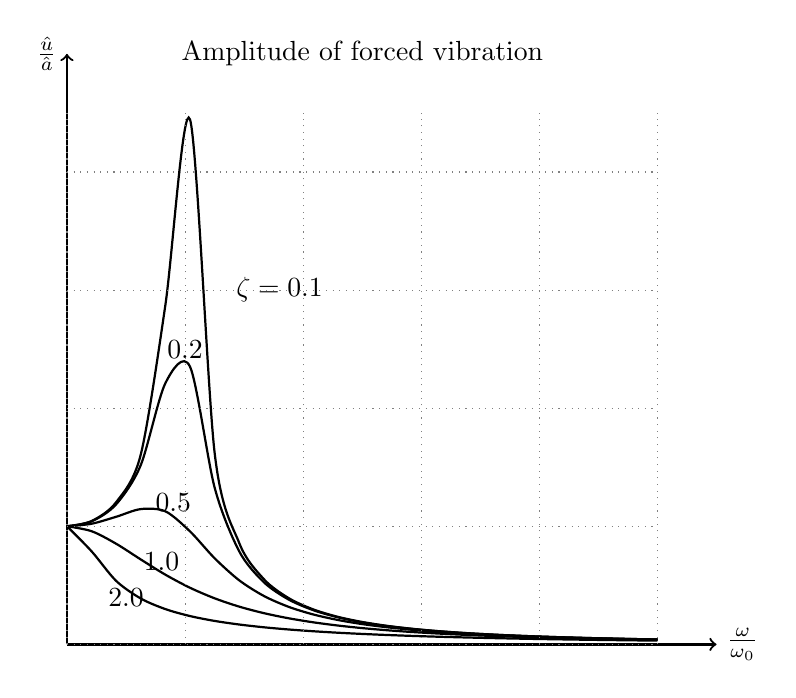
\begin{tikzpicture}[scale=1.5]
    \draw[->, black, thick] (0,0) -- (5.5,0) node[right] {$\frac{\omega}{\omega_0}$};
    \draw[->, black, thick] (0,0) -- (0, 5) node[left] {$\frac{\hat{u}}{\hat{a}}$};
    

    \draw[domain = 0:5, color = black, thick] plot[smooth] (\x,{1 / sqrt((1-\x^2)^2 + (2*0.1*\x)^2)}) node at (1.8, 3) {$\zeta = 0.1$};
    \draw[domain = 0:5, color = black, thick] plot[smooth] (\x, {1 / sqrt((1-\x^2)^2 + (2*0.2*\x)^2)}) node at (1, 2.5) {$0.2$};
    \draw[domain = 0:5, color = black, thick] plot[smooth] (\x, {1 / sqrt((1-\x^2)^2 + (2*0.5*\x)^2)}) node at (0.9, 1.2) {$0.5$};
    \draw[domain = 0:5, color = black, thick] plot[smooth] (\x, {1 / sqrt((1-\x^2)^2 + (2*1.0*\x)^2)}) node at (0.8, 0.7) {$1.0$};
    \draw[domain = 0:5, color = black, thick] plot[smooth] (\x, {1 / sqrt((1-\x^2)^2 + (2*2.0*\x)^2)}) node at (0.5, 0.4) {$2.0$};
    
    %Grid
    \draw[gray, dotted] grid (5,4.5);
    
    \node at (2.5, 5) {Amplitude of forced vibration};
\end{tikzpicture}

    \begin{minipage}[t]{.49\linewidth}
        geg.:
        \begin{tasks} (1)
            \task[] $m = \SI{3}{\kilo\gram}$
            \task[] $\omega_{gemessen} = \SI{10}{\radian\per\second}$
            \task[] $0 < \zeta < 1$
            \task[] $\zeta_{gemessen} = 0.1$
        \end{tasks}
        \end{minipage}
        \begin{minipage}[t]{.49\linewidth}
        ges.:
        \begin{tasks}
            \task$k$
        \end{tasks}
    \end{minipage}\\
    \vspace{1cm}

    \underline{Zusatzfrage:} Je nach Messprinzip, wird entweder die ungedämpfte
    Eigenfrequenz, die gedämpfte Eigenfrequenz oder die maximale Anwortamplitude
    hervorrufende Anregungsfrequenz direkt erfasst. Wie groß ist für $\zeta = 0.1$ der
    Fehler bei der Schätzung von $k$, wenn man diese Frequenzen gleichsetzt?

    \begin{solution}
        \begin{alignat*}{2}
            &\text{ungedämpfte Eigenkreisfrequenz  } \omega_0 = \sqrt{\frac{k}{m}} \\
            &k_{ungedaempft} = m \cdot \omega_{gemessen}^2 &&= \SI{300.000}{\newton \per \meter} \\
            &\text{gedaempfte Eigenfrequenz  } \omega_1 = \omega_0 \sqrt{1-\zeta^2} \\
            &\omega_{gedaempft} = \frac{\omega_{gemessen}}{\sqrt{1-\zeta_{gemessen}^2}} &&= 10.05\\
            &k_{gedaempft} = m \cdot \omega_{gedaempft}^2 &&= \SI{303.030}{\newton \per \meter}\\
            &\Delta = 100 \cdot \frac{|k_{gedaempft} - k_{ungedaempft}|}{k_{ungedaempft}} &&= 1.01 \%\\
            &\text{maximale Antwortamplitude bei der Anregungsfrequenz  } \omega_{MA} = \omega_0 \sqrt{1-2 \zeta^2} \\
            &\omega_{MA} = \frac{\omega_{gemessen}}{\sqrt{1-2\zeta_{gemessen}^2}} &&= 10.102\\
            &k_{MA} = m \cdot \omega_{MA}^2 &&= \SI{306.122}{\newton \per \meter}\\
            &\Delta = 100 \cdot \frac{|k_{MA} - k_{ungedaempft}|}{k_{ungedaempft}} &&= 2.04 \% \\ 
        \end{alignat*}
    \end{solution}

